% !TeX spellcheck = en_GB
\begin{figure}[!t]
	\centering
	%    \begin{subfigure}[b]{\textwidth}
	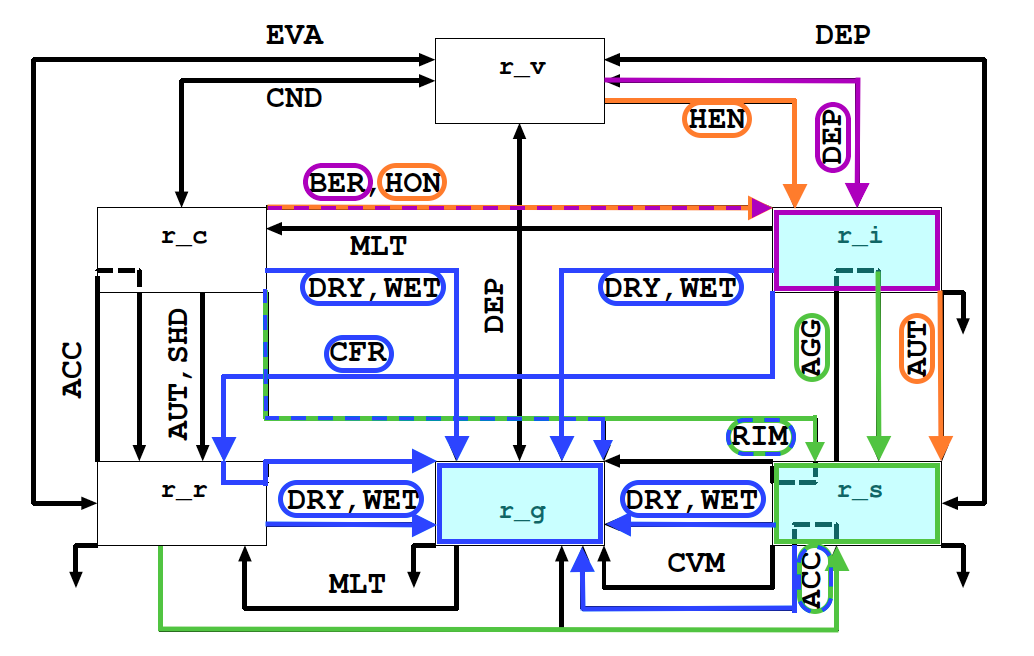
\includegraphics[width=\textwidth]{./fig_MEPS/ICE3_scheme_copy}
	%	\end{subfigure}
	\caption{Microphysical processes for mixed phase clouds in the ICE3 scheme in AROME \citep[adapted from ][]{meteo_france_meso-nh_2009}. %In orange the initiation processes for primary ice r$_i$ and snowflakes r$_s$. The growing processes of r$_i$ is shown in purple and for r$_s$ in green. Graupel particles, r$_g$, grow from existent particles and the processes are shown in blue. 
    Orange lines show the initiation of pristine ice crystals and snowflakes ($\mathbf{s}$). Purple  lines and boxes present the growth mechanisms of $\mathbf{i}$ (BER, DEP). Green lines demonstrate the expansion of the snowflakes (RIM, AGG, ACC). Graupel ($\mathbf{g}$) forms as an effect of heavy riming (RIM) by collision of larger raindrops with snowflakes (ACC), WET/DRY growth or contact freezing of raindrops (CFR). All graupel growth processes are indicated by blue lines were hail formation is included. 
    }\label{fig:ICE3_scheme}
\end{figure}